\begin{center}
        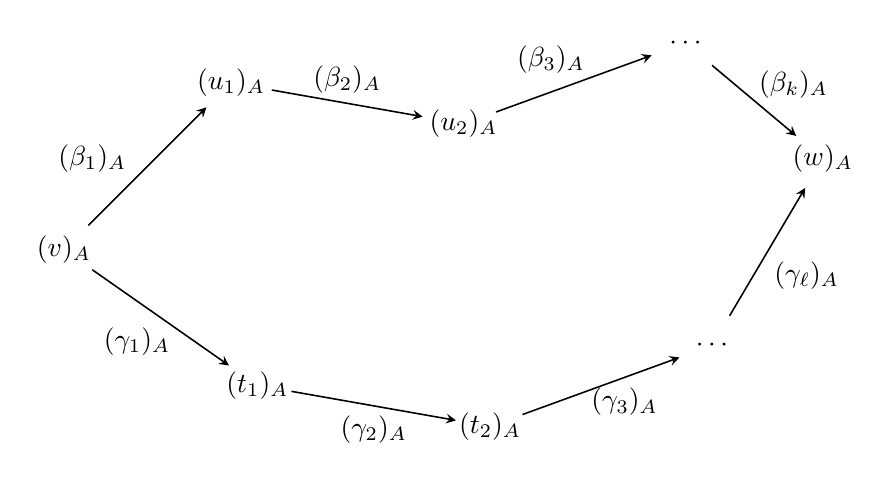
\begin{tikzpicture}[line width = 0.2mm, >=stealth, shorten >= 12.5pt, shorten <=12.5pt]
            \draw[->, Black] (0,0) coordinate (a)
            -- node[above, xshift = -0.7cm, yshift = -0.2cm] {$(\beta_1)_A$}
             ++(45:3) coordinate (b);
            \draw[->, Black,  shorten >= 15pt, shorten <=15pt] (b)
            -- node[above] {$(\beta_2)_A$}
             ++(-10:3) coordinate (c);
            \draw[->, Black, shorten >= 13pt] (c)
            -- node[above, xshift = -0.3cm] {$(\beta_3)_A$}
             ++(20:3) coordinate (d);
            \draw[->, Black] (d)
            -- node[above, xshift = 0.5cm, yshift = -0.1cm] {$(\beta_k)_A$}
            ++(-40:2.275) coordinate (e);
            \node at (a) {$(v)_A$};
            \node at (b) {$(u_1)_A$};
            \node at (c) {$(u_2)_A$};
            \node at (d) {$\cdots$};
            \node at (e) {$(w)_A$};
    
            \draw[->, Black] (0,0)
            -- node[below, xshift = -0.3cm] {$(\gamma_1)_A$}
            ++(-35:3) coordinate (f);
            \draw[->, Black] (f)
            -- node[below] {$(\gamma_2)_A$}
            ++(-10:3) coordinate (g);
            \draw[->, Black, shorten >= 12.5pt] (g)
            -- node[below, xshift = 0.3cm, yshift = 0.1cm] {$(\gamma_3)_A$}
            ++(20:3) coordinate (h);
            \draw[->, Black] (h)
            -- node[below, xshift = 0.5cm] {$(\gamma_{\ell})_A$}
             (e);
            \node at (f) {$(t_1)_A$};
            \node at (g) {$(t_2)_A$};
            \node at (h) {$\cdots$};
        \end{tikzpicture}
    \end{center}